\chapter{Introduzione}

\begin{center}
    ``Without data you're just another person with an opinion.''

    - W. Edward Deming, Data Scientist
\end{center}
Senza misure non è possibile produrre i risultati attesi, misurare i miglioramenti e quantificare il successo.\
Il traffico di rete non fa eccezione a questa regola.\
\begin{center}
    ``If you can't measure it, you can't improve it.''

    (Lord Kelvin, 1824 – 1907)

\end{center}
\begin{center}
    ``If you can't measure it, you can't manage it.''

    (Peter Drucker, 1909 – 2005)
\end{center}

\subsubsection{Come si misura il traffico di rete}

Individuare un punto della rete dove passa il traffico da analizzare (tipicamente vicino al router) e installarvi una \textbf{sonda di rete} capace di analizzare tale traffico:
\begin{itemize}
    \item \textbf{Passiva}:\ solo analisi, no modifica/blocco traffico.
    \item \textbf{Attiva}:\ il traffico attraversa la sonda che può bloccarlo se necessario.
\end{itemize}
\begin{figure}[H]
    \centering
    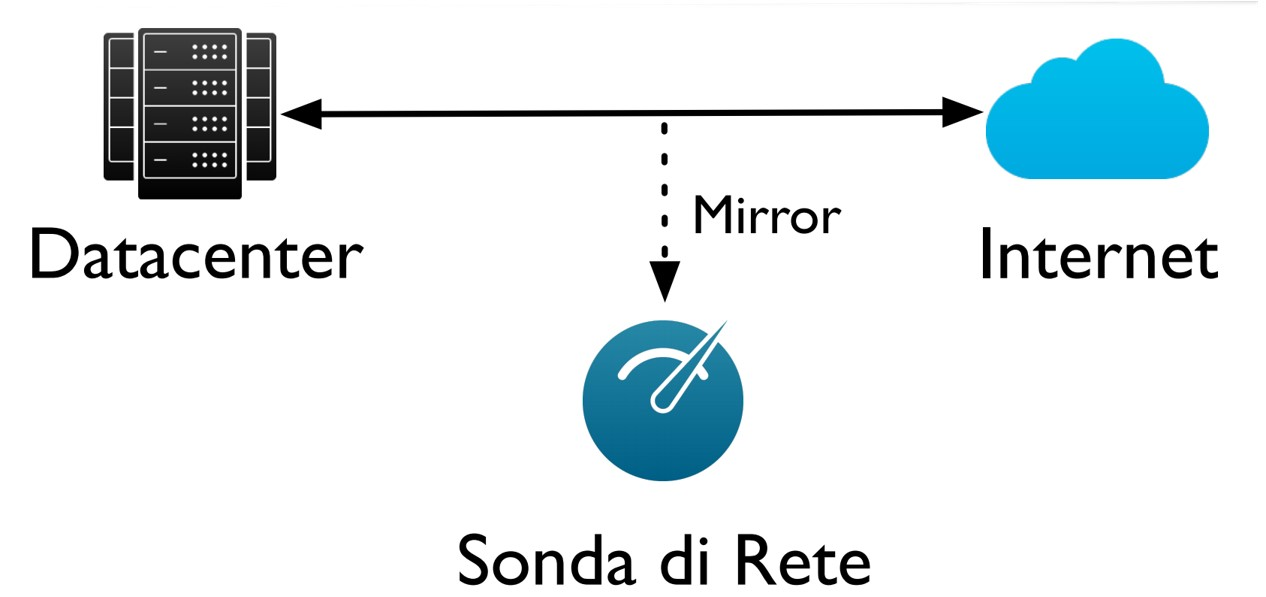
\includegraphics[width=0.6\textwidth]{immagini/Sonda_rete.jpg}
\end{figure}

\subsubsection{Che misure di rete possiamo fare?}

Analisi \textbf{quantitativa} di traffico
\begin{itemize}
    \item Top Talkers (Senders and Receivers).
    \item Destinazioni verso/da le quali viene scambiato traffico.
    \item Protocolli applicativi utilizzati (Skype, HTTP, Email).
    \item Rendicontazione traffico per host.
\end{itemize}
Analisi \textbf{qualitativa} di traffico
\begin{itemize}
    \item Utilizzo di traffico non permesso (es.\ Tor o VPN anonime).
    \item Identificazione errori ed anomalie di rete che possono causare malfunzionamenti nell'utilizzo dei servizi di rete.
\end{itemize}

\subsubsection{Gestione di Rete}

Dal punto di vista del monitoraggio una rete è divisa in due grandi categorie:\
\begin{itemize}
    \item \textbf{Element management}:\ gestione dei device e delle periferiche.
    \item \textbf{Analisi dei dati}:\ analisi del traffico di rete.
\end{itemize}

\section{Motivazioni}

Situazione attuale:
\begin{itemize}
    \item le ``informazioni'' acquisiscono un crescente significato come risorse strategiche.
    \item una rete di computer non è più solo un elemento di supporto in un'impresa, ma assume sempre più frequentemente una posizione chiave.
    \item il numero di computer interconnessi è aumentato notevolmente negli ultimi anni.\ Questo processo probabilmente continuerà a persistere.
    \item la complessità e la funzionalità dei componenti cresce in corrispondenza delle prestazioni dell'hardware disponibile.
\end{itemize}
Richiesta:
\begin{itemize}
    \item Disponibilità permanente dei servizi di rete con qualità ottimale.
    \item Riduzione dei costi per l'infrastruttura di rete dell'azienda.
\end{itemize}
Necessità:\ gestione assistita da computer di reti eterogenee.

\section{Network Management Dimensions}

L'\textbf{element management} si divide in tre parti:\ la \textbf{dimensione funzionale}, la \textbf{dimensione del tempo} e la \textbf{dimensione dell'oggetto}.\
\begin{figure}[H]
    \centering
    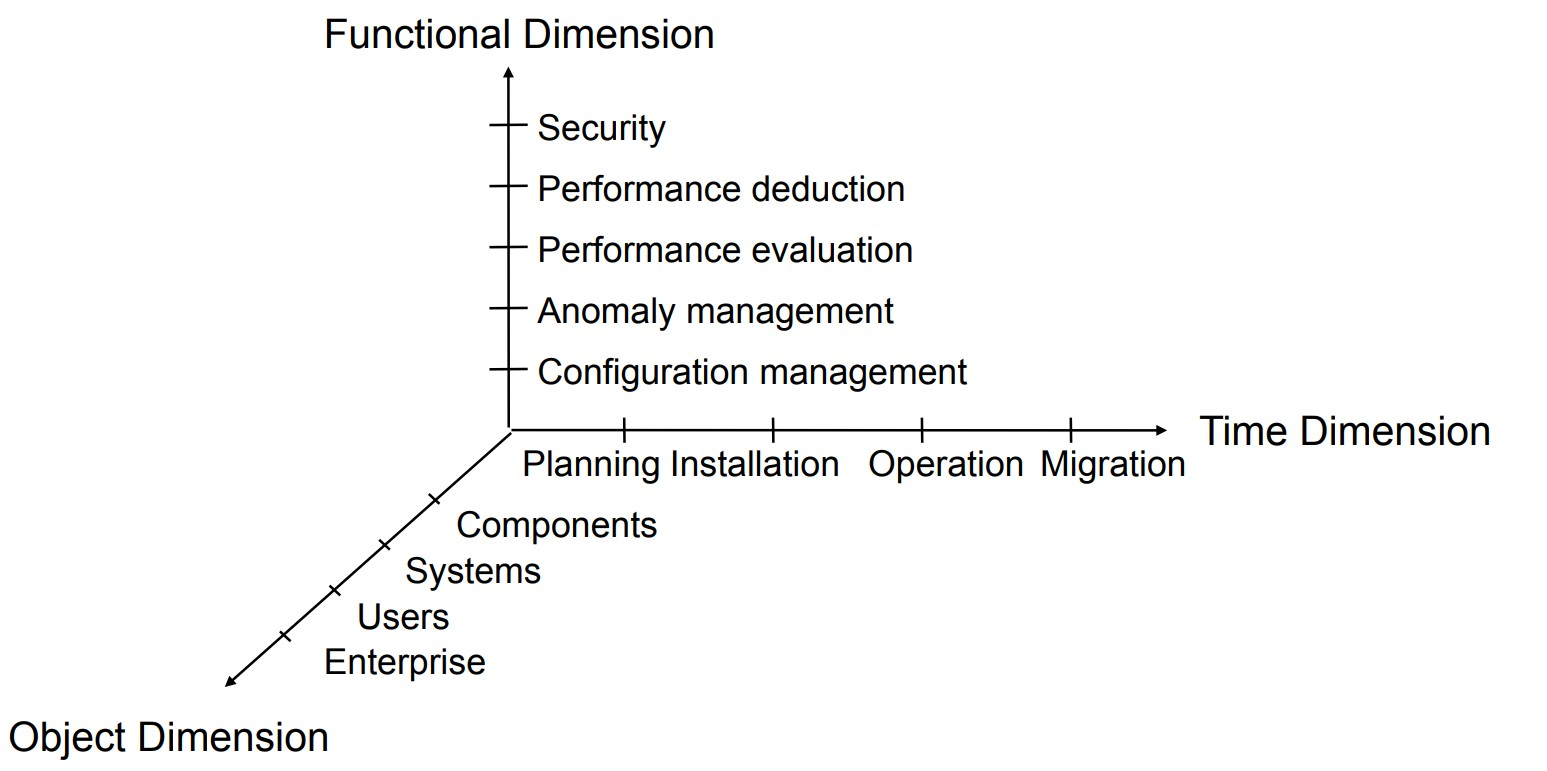
\includegraphics[width=\textwidth]{immagini/NetworkManagementDimension.jpg}
\end{figure}

\noindent La \textit{dimensione funzionale} fornisce informazioni sulle funzionalità svolte da un determinato componente.\
Gli aspetti di un componente di rete che devono essere considerati sono:

\begin{itemize}
    \item \textbf{Gestione della configurazione}:\ capacità di impostare delle opzioni di funzionamento di un oggetto.\ Deve essere resa disponibile a chi vi interagisce:\ è necessaria ogni volta che c'è un problema.
    \item \textbf{Gestione di un'anomalia}:\ definire una base line, ossia capire il comportamento medio della rete, e controllare se il comportamento è stabile nel tempo.\ Ci sono due strade (di solito perseguite contemporaneamente) per individuare le anomalie:\ andare a \textit{definire dei paletti} oltre i quali le attività sono considerate errate o andare a \textit{definire delle metriche} per osservare quanto il comportamento atteso si discosta dal comportamento attuale.\ L'anomalia deve essere messa in relazione anche a fattori esterni come il numero di utenti che usano la rete, il periodo/stagione.
    \item \textbf{Valutazione della performance}:\ è una misura utile all'operatore per riuscire a capire se la rete funziona correttamente.
    \item \textbf{Deduzione della performance}:\ riuscire a creare un'aspettativa rispetto al futuro.\ Conoscendo la rete e conoscendo il comportamento degli utenti è possibile prevedere le performance future.\
    \item \textbf{Sicurezza}:\ far sì che la rete funzioni in maniera sicura.\ Se siamo un operatore non ci possiamo chiedere se tutti gli utenti utilizzino protocolli non sicuri, ma ci dobbiamo occupare di quei casi che creano problemi a tutti.
\end{itemize}

\noindent La \textit{dimensione del tempo} è necessaria a chi costruisce la rete per prevedere le operazioni future che vi verranno fatte.

La \textit{dimensione dell'oggetto} ha come obiettivo il bilanciamento della rete per garantire il funzionamento ottimale.

\section{Terminologia e concetti fondamentali}

Il controllo, il coordinamento e il monitoraggio delle risorse avviene tramite la manipolazione dai cosiddetti \textbf{managed objects}:
\begin{center}
    ``\textit{Un managed object è la vista astratta di una risorsa che presenta le sue proprietà come viste dalla (e ai fini della) gestione}.'' (ISO 7498-4)
\end{center}
I managed objects sono una rappresentazione astratta di una risorsa reale.\
Il confine di un managed object specifica quali dettagli sono accessibili a un sistema di gestione e quali sono schermati (black box).\
\begin{figure}[H]
    \centering
    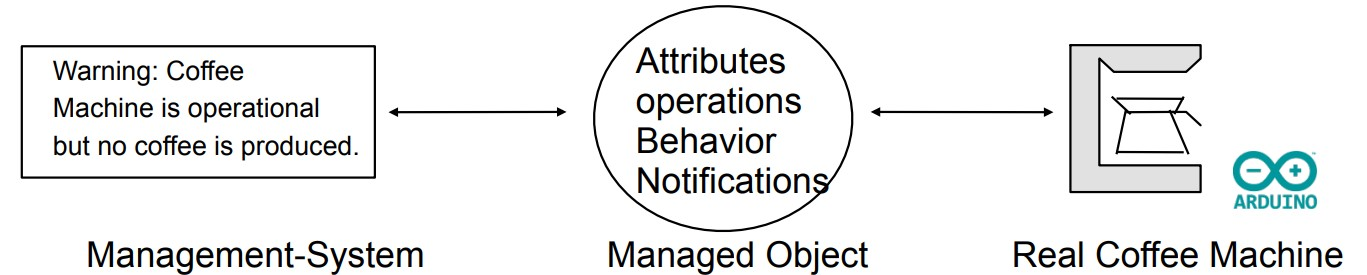
\includegraphics[width=\textwidth]{immagini/MO.jpg}
\end{figure}
\noindent I managed objects non corrispondono necessariamente agli oggetti, come si sa dalla programmazione orientata agli oggetti.\
Le variabili semplici corrispondono ai MO nella gestione di Internet.\

\subsection{Managed Objects}

Gli \textbf{attributi} descrivono lo stato, la condizione, degli oggetti gestiti:\ possono cambiare quando cambia la condizione dell'oggetto reale e possono essere manipolati mediante \textbf{operazioni} di gestione.\
Quest'ultime hanno lo scopo di rendere possibile l'accesso a un oggetto gestito e tipicamente sono operazioni di \texttt{get}, \texttt{set}, \texttt{create} e \texttt{delete}.\
Si noti che il numero e il tipo di operazioni influenzano le prestazioni e la complessità dell'oggetto.

Il \textbf{comportamento} dei managed objects è normalmente definito in un inglese semplice e determina la semantica e l'interazione con la risorsa reale.\

Inoltre vengono definite delle \textbf{notifiche}, messaggi che possono essere generati da un managed object quando si verificano situazioni specifiche.

\subsection{Management Information Base (MIB)}

L'unione di tutti i managed objects contenuti in un sistema costituisce il \textbf{Management Information Base} (\textbf{MIB}) del sistema:
\begin{center}
    ``\textit{L'insieme di managed objects all'interno di un sistema, insieme ai loro attributi, costituisce il management information base di quel sistema}.''\\(ISO 7498-4)
\end{center}
\begin{figure}[H]
    \centering
    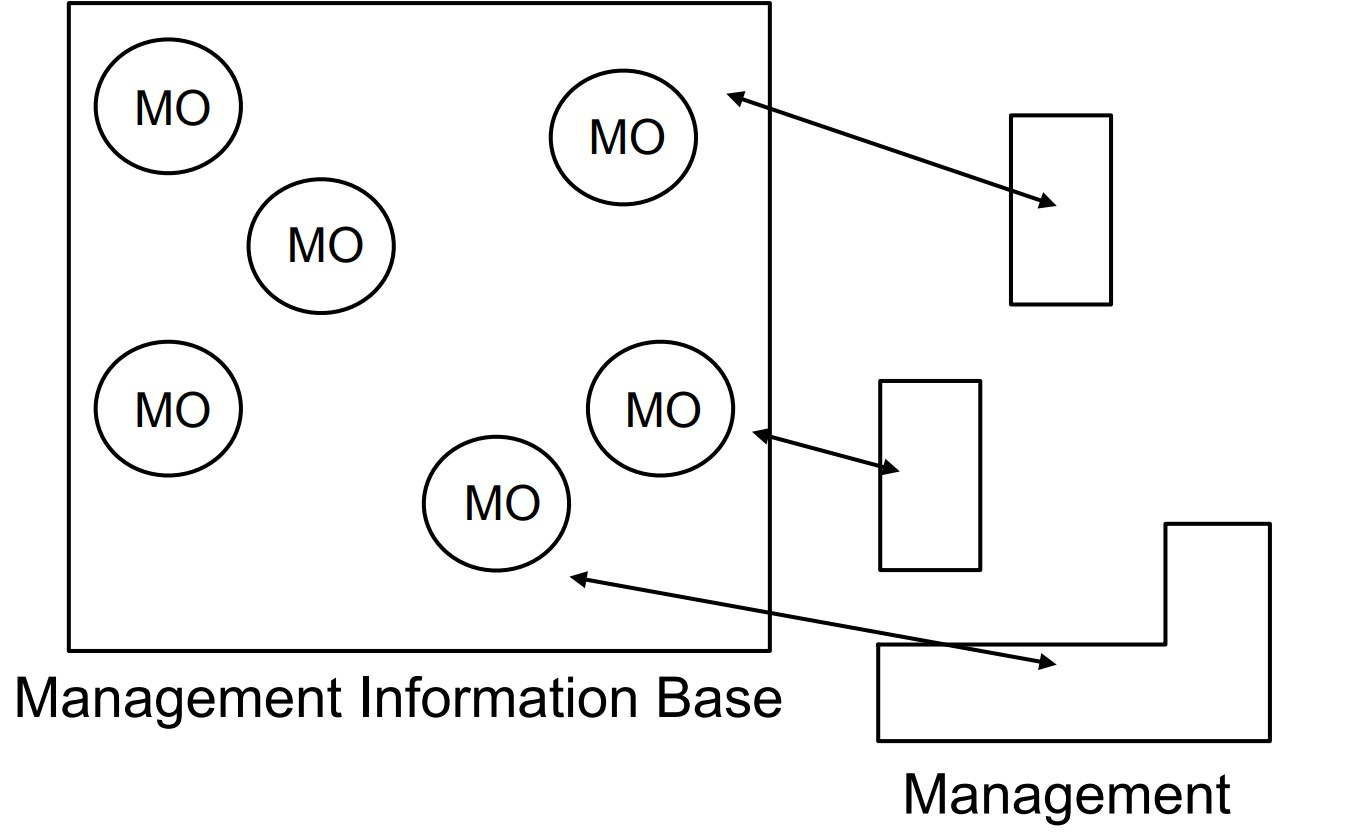
\includegraphics[width=0.7\textwidth]{immagini/MIB.jpg}
\end{figure}
Un MIB dovrebbe essere noto sia all'implementatore che al manager.\

\subsubsection{MIB Modularity}

I managed objects di un sistema sono generalmente definiti in più definizioni MIB utilizzando un linguaggio di specifica.\
I moduli sono stati introdotti nei MIB per consentire la modularità del design, infatti diversi moduli possono essere definiti da diversi team e la funzionalità di gestione può essere gradualmente estesa e modificata (anche mediante MIB proprietari).\
Sistemi diversi possono supportare diversi moduli/versioni MIB.

\subsection{Manager/Agent Paradigm}

L'agent implementa i MOs MIB accedendo alle risorse reali ed elabora le richieste di un manager al quale trasmette le risposte appropriate.\
Quindi protegge i MOs da accessi non autorizzati utilizzando le regole di controllo dell'accesso e l'autenticazione della comunicazione con il partner ed invia notifiche su importanti cambiamenti di stato nel MIB.

Il manager, invece, è colui che esercita il controllo (controlla le funzioni) ed è quindi l'istanza cruciale:\ può avviare operazioni di gestione mediante appropriate operazioni di protocollo per la manipolazione di MO.\
Il suo compito è ricevere messaggi dagli agenti e trasmetterli (per la gestione) alle applicazioni appropriate.

\subsubsection{Management Protocol}

Le applicazioni di gestione e i MO spesso non sono sullo stesso nodo:\ l'agent gira all'interno della risorsa, parla con la parte fisica di quest'ultima e rimane in ascolto in attesa di richieste; il manager invece sta fuori dalla risorsa (sta all'interno del manager di sistema) e invia i comandi all'agent.\
I manager identificheranno gli agent e la risorsa in base all'indirizzo IP e la porta.\
Un \textbf{management protocol} implementa l'accesso agli oggetti gestiti a distanza codificando i dati di gestione che vengono poi protetti durante il trasferimento.

\begin{figure}[H]
    \centering
    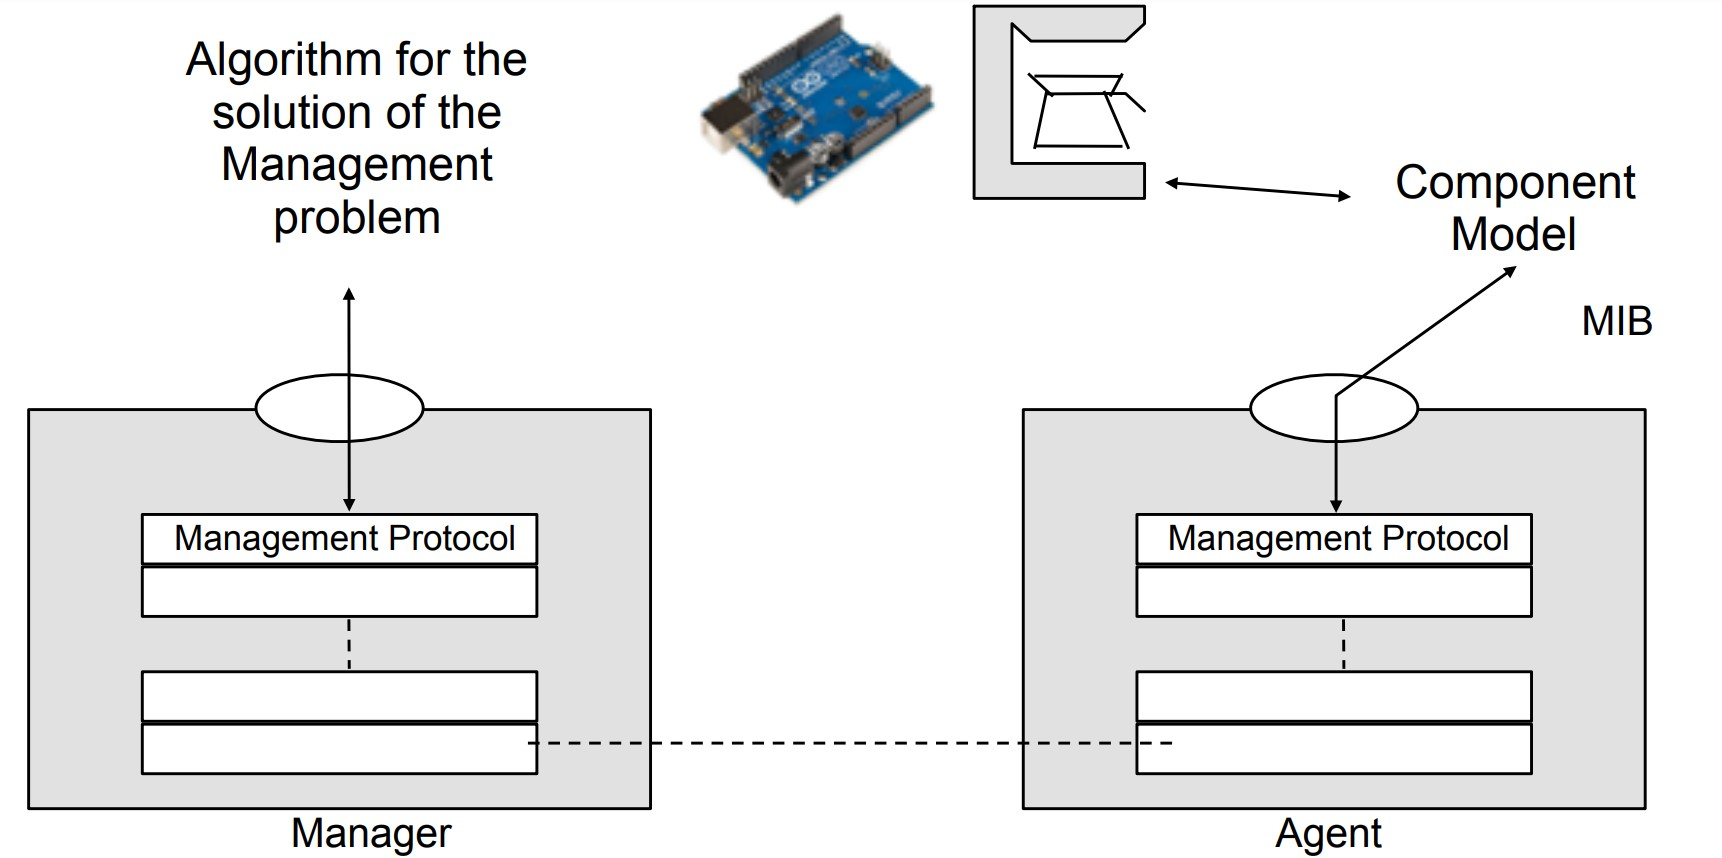
\includegraphics[width=\textwidth]{immagini/ManagementProtocol.jpg}
\end{figure}

\subsection{Functional Areas (FCAPS)}

Le applicazioni gestionali possono essere suddivise in cinque aree funzionali:
\begin{itemize}
    \item \textbf{Fault manager}:\ rilevamento, isolamento e riparazione degli errori.
    \item \textbf{Configuration manager}:\ produzione e amministrazione delle informazioni di configurazione, amministrazione dei nomi, avvio, verifica e cessazione dei servizi.
    \item \textbf{Account management}:\ inserimento dei dati di consumo (utilizzo), distribuzione e monitoraggio dei contingenti, fatturazione cliente per consumo di risorse.
    \item \textbf{Performance management}:\ raccolta dati statistici, determinazione delle prestazioni del sistema, modifiche ai sistemi per aumentare l'efficienza.
    \item \textbf{Security management}:\ produzione e verifica delle policy di sicurezza, generazione e distribuzione di password e account, report e analisi di eventi rilevanti per la sicurezza.
\end{itemize}

\noindent Queste cinque aree funzionali sono identificate tramite l'acronimo FCAPS.\
Le aree non sono reciprocamente indipendenti (la misurazione dei dati ha spesso un impatto sulla configurazione del sistema).\
Le funzioni di base (ad esempio il monitoraggio di un contatore per i valori di soglia) risiedono spesso in diverse aree funzionali.

\subsection{Management Architectures Overview}

La struttura delle informazioni di gestione definisce le regole della descrizione dei Managed Objects:
\begin{itemize}
    \item Identificazione e designazione di MOs.
    \item Composizione dei MO.
    \item Comportamento dei MO.
    \item Rapporti con altri MO.
    \item Possibili operazioni e messaggi interni dei MO.
\end{itemize}
Quindi, contiene la definizione dei tipi di dati, della struttura e della sintassi per la descrizione dei MO.\
La quantità delle descrizioni dei MO in conformità a queste regole definisce il \textit{Management Information Base} (MIB).

I protocolli e servizi di gestione definiscono i servizi e abilitano l'accesso ai MO remoti.\
Possono essere utilizzati diversi protocolli per l'implementare i servizi definiti:\ la primitiva del servizio e le operazioni del protocollo appropriato influenzano notevolmente l'efficienza e la complessità del sistema di gestione.

\subsection{Servizi e protocolli: alcune definizioni}

\textbf{Servizio}:\ definito come una funzione astratta fornita da una rete.

\noindent\textbf{Primitiva di servizio}:\ le singole funzioni elementari sono chiamate primitive di servizio.\
I servizi ISO/OSI tipici sono:
\begin{table}[H]
    \centering
    \begin{tabular}{l l}
        \texttt{request}    & richiesta di servizio                              \\
        \texttt{indication} & indicazione che è stato richiesto un servizio      \\
        \texttt{response}   & reazione del servizio a una richiesta di servizio  \\
        \texttt{confirm}    & conferma che è stato fornito un servizio richiesto \\
    \end{tabular}
\end{table}
\noindent\textbf{Service Access Point} (\textbf{SAP}):\ l'interfaccia su cui la primitiva del servizio può accedere come punto di accesso al servizio.

\noindent\textbf{Entità}:\ i servizi forniti dalle cosiddette istanze.

\noindent\textbf{Protocollo}:\ le regole e le restrizioni in base alle quali le istanze interagiscono con altre istanze.

\subsection{Rappresentazione e stratificazione dei servizi}

La definizione degli strati è un principio fondamentale per la strutturazione dei sistemi di comunicazione.\
I servizi di uno strato possono accettare solo primitive di servizio di servizi in strati adiacenti.
\begin{figure}[H]
    \centering
    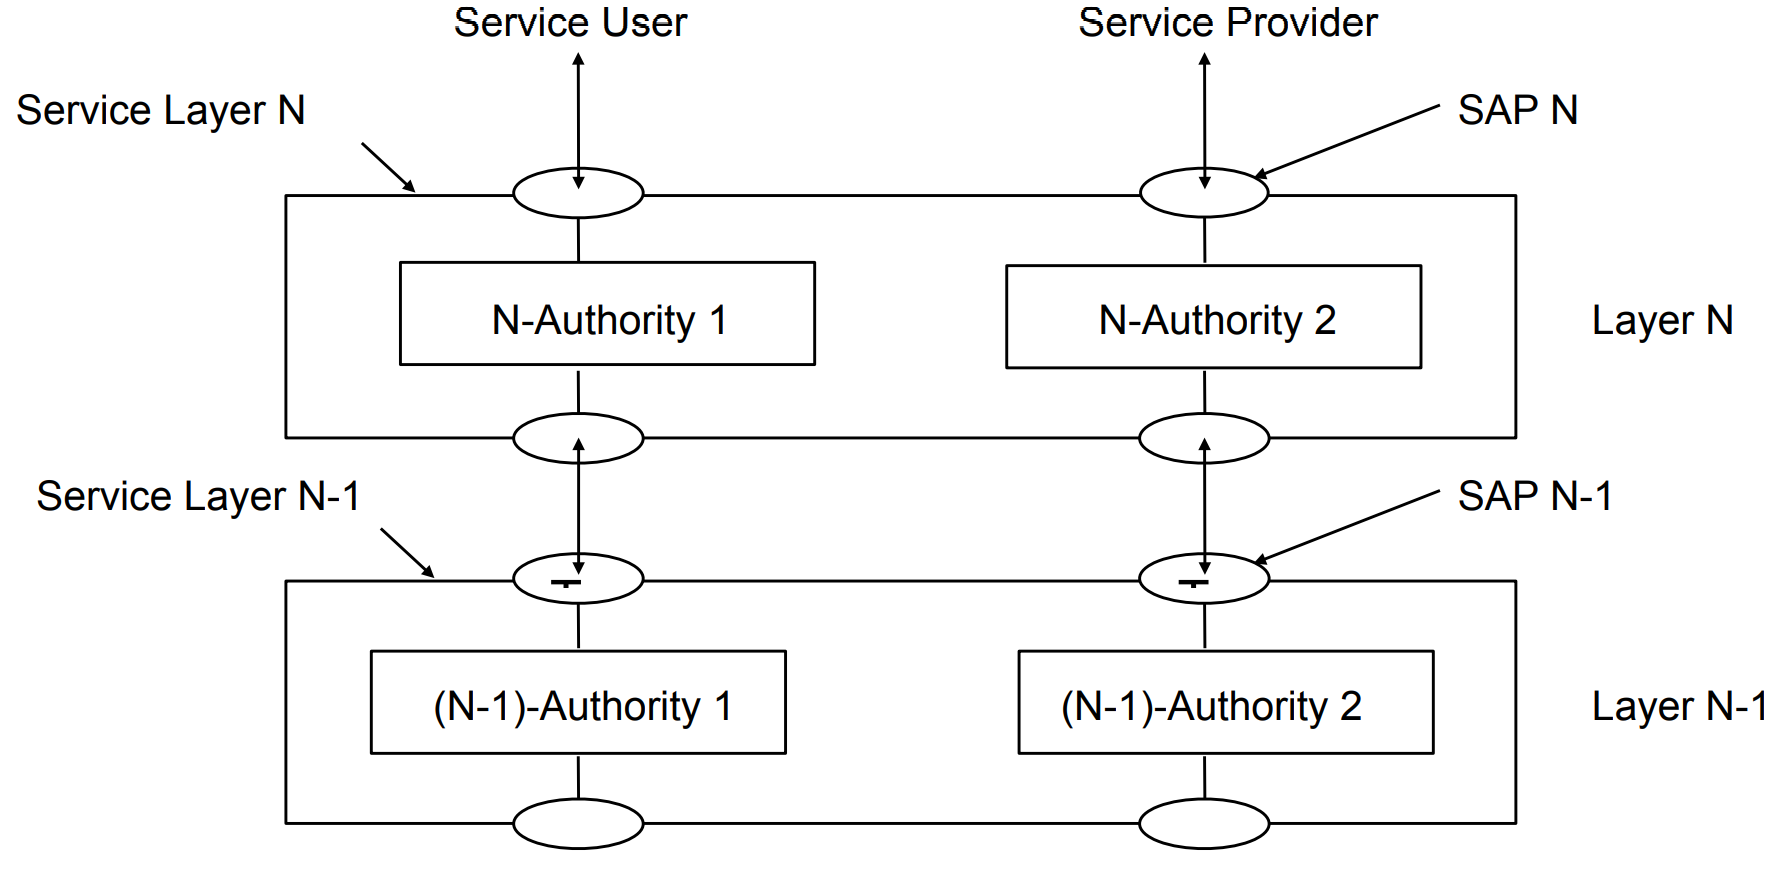
\includegraphics[width=0.7\textwidth]{immagini/Layering_services.png}

\end{figure}

\subsection{Time Diagrams}

I diagrammi temporali chiariscono le connessioni temporali e spaziali tra le primitive di servizio.

I servizi si suddividono in due gruppi, \textit{confermati} e \textit{non confermati}.\
Un \textbf{servizio confermato} è tale se a fronte di una richiesta manda una risposta contenente l'esito dell'esecuzione della primitiva.\
Un servizio è \textbf{non confermato} se a fronte di una richiesta non viene mandata nessuna risposta.\

\begin{figure}[H]
    \centering
    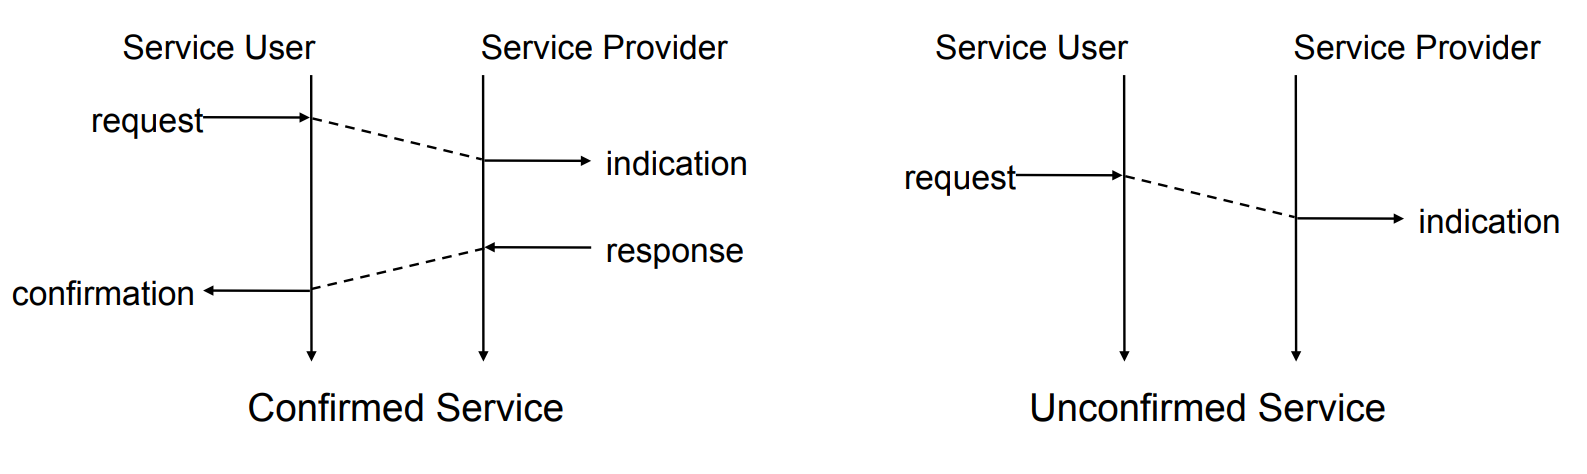
\includegraphics[width=\textwidth]{immagini/TimeDiagrams.png}
\end{figure}

\noindent L'asse verticale è l'asse del tempo, l'asse orizzontale fornisce la distanza spaziale tra utenti e fornitori di servizi.\
Le richieste di servizio di un servizio confermato possono comportare una conferma positiva o negativa.\
Le richieste di servizio di un servizio non confermato non vengono riconosciute.

In entrambi i casi ciò che il mittente invia, spesso, non è uguale a ciò che il destinatario riceve.\
Si consideri il caso di messaggistica:\ quando il mittente scrive il messaggio specifica il numero del destinatario; quest'ultimo quando riceve il messaggio non visualizza il proprio numero, bensì quello del mittente (oltre ad una serie di informazione aggiuntive come ad esempio la data).\
Alcuni protocolli come \texttt{http} possono infatti modificare il payload del messaggio, soprattutto con l'utilizzo dei proxy http; altri protocolli come \texttt{smtp} invece estendono gli header dei messaggi.\
In linea generale tutti i protocolli di tipo ``store-and-forward'' eseguono delle alterazioni al messaggio, per questa ragione nei time diagrams ``\texttt{request}'' e ``\texttt{indication}'' assumono connotati diversi.\

Si noti che quando due entità devono comunicare devono usare un meccanismo di serializzazione/codifica in modo tale che le richieste e le risposte siano riconosciute da entrambe le parti.\
Nel mondo delle reti è necessario mantenere il minor numero di informazioni aggiuntive al dato, così da sprecare meno spazio possibile per la codifica/decodifica dei dati (per questa ragione spesso vengono mandate informazioni in formato compresso).\

\subsection{ISO/OSI-Reference Model}

\begin{figure}[H]
    \centering
    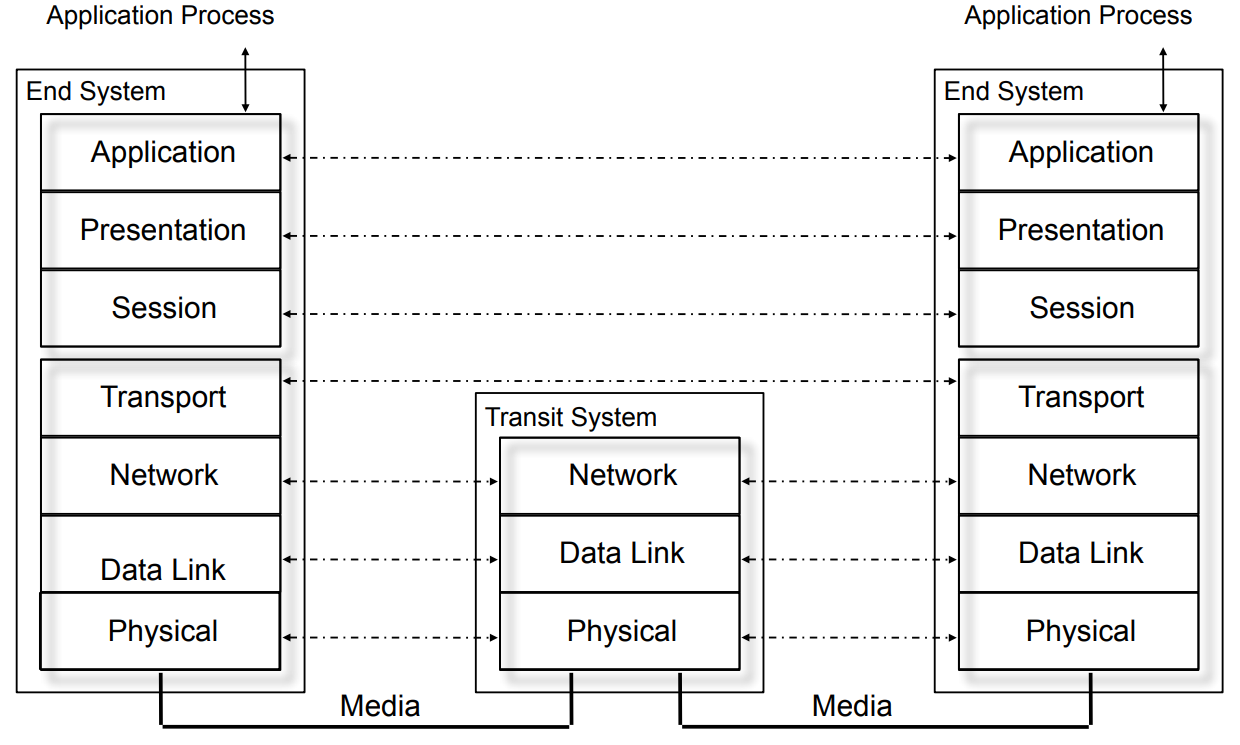
\includegraphics[width=0.9\textwidth]{immagini/ISO_OSI.png}
\end{figure}

\noindent La pila ISO/OSI presenta sette livelli, i primi tre vengono definiti ``\textit{livelli di presentation}'' e sono utili per lo scambio corretto dei messaggi e per la gestione del loro formato tra applicazioni diverse.\
I dispositivi intermedi di rete presentano solo gli ultimi tre livelli della pila ISO/OSI.\
La rete in questo caso deve essere a conoscenza di tutto (anche dei formati diversi inviati sulla rete stessa).

\begin{table}[H]
    \centering
    \begin{tabular}{|c|m{22.7em}|}
        \hline
        \multicolumn{2}{|c|}{\textit{ISO/OSI Higher Layers}}                                                                                                                                                                                                                                                                                                         \\\hline\hline
        \textbf{Session Layer}      & Sincronizzazione e coordinamento dei processi comunicativi.\newline Controllo della sessione (checkpoint per il ripristino).                                                                                                                                                                                                   \\\hline
        \textbf{Presentation Layer} & Trasformazione e adattamento delle presentazioni dei dati (es ASCII EBCDIC). \newline Serializzazione delle strutture dati ai fini del trasferimento. \newline Compressione dati.                                                                                                                                              \\\hline
        \textbf{Application Layer}  & Fornitura di servizi fondamentali, utilizzabili direttamente da qualsiasi applicazione inclusi (ma non limitati a):\ trasferimento di file, terminali virtuali, amministrazione dello spazio dei nomi, accesso al database, gestione della rete, reti di comunicazione elettronica, controllo del processo e della stampa\dots \\\hline
    \end{tabular}
\end{table}

\begin{table}[H]
    \centering
    \begin{tabular}{|c|m{22.7em}|}
        \hline
        \multicolumn{2}{|c|}{\textit{ISO/OSI Transport System}}                                                                                                                                                                                                                                                                                                                     \\\hline\hline
        \textbf{Physical Layer}  & Trasporto di un flusso di bit su un supporto.\newline Trasporto a seconda delle caratteristiche del supporto utilizzato.\newline Rappresentazione dei valori 0 e 1 (es.\ livelli di tensione). \newline Sincronizzazione tra mittenti e destinatari. \newline Definizione di spine standard per l'interconnessione dei media.                    \\\hline
        \textbf{Data Link Layer} & Trasporto di un frame di bit.\newline Comunicazione dati tra sistemi che condividono un media comune.\newline Rilevamento e ripristino degli errori di trasferimento. \newline Controllo del flusso per gestire i picchi di traffico (congestione).\newline Implementazione solitamente in hardware su schede adattatrici (es. Scheda Ethernet). \\\hline

        \textbf{Network Layer}   & Determinazione di un percorso attraverso la rete (routing).\newline Multiplex di connessioni di rete su una connessione condivisa. \newline Rilevamento e ripristino degli errori tra i sistemi finali. \newline Controllo del flusso tra sistemi finali. \newline Divisione di un pacchetto in più frame.                                       \\\hline
        \textbf{Transport Layer} & Comunicazione end-to-end tra le applicazioni. \newline Connessioni virtuali su servizi di datagramma senza connessione.\newline spesso Rilevamento e ripristino degli errori tra le applicazioni.\newline Controllo del flusso tra le applicazioni.\newline Utilizzo simultaneo di più servizi.                                                  \\\hline
    \end{tabular}
\end{table}

\subsection{Internet Layer Model}

\noindent Nel mondo Internet sono presenti molti meno livelli nella pila dei protocolli, questo perché molti problemi non vengono più demandati alla rete.\
Se si considera il caso di scambio di file in diversi formati, tali informazioni non necessitano di essere presenti sulla rete come nel caso del modello ISO/OSI, ma sono gestite a livello applicativo:\ solo le applicazioni necessitano di essere compatibili tra di loro, non l'intera parte sottostante.\
Il modello di Internet a livello di gestione è molto più semplice del modello ISO/OSI, questo è possibile notarlo anche nell'ambito della standardizzazione.

\begin{figure}[H]
    \centering
    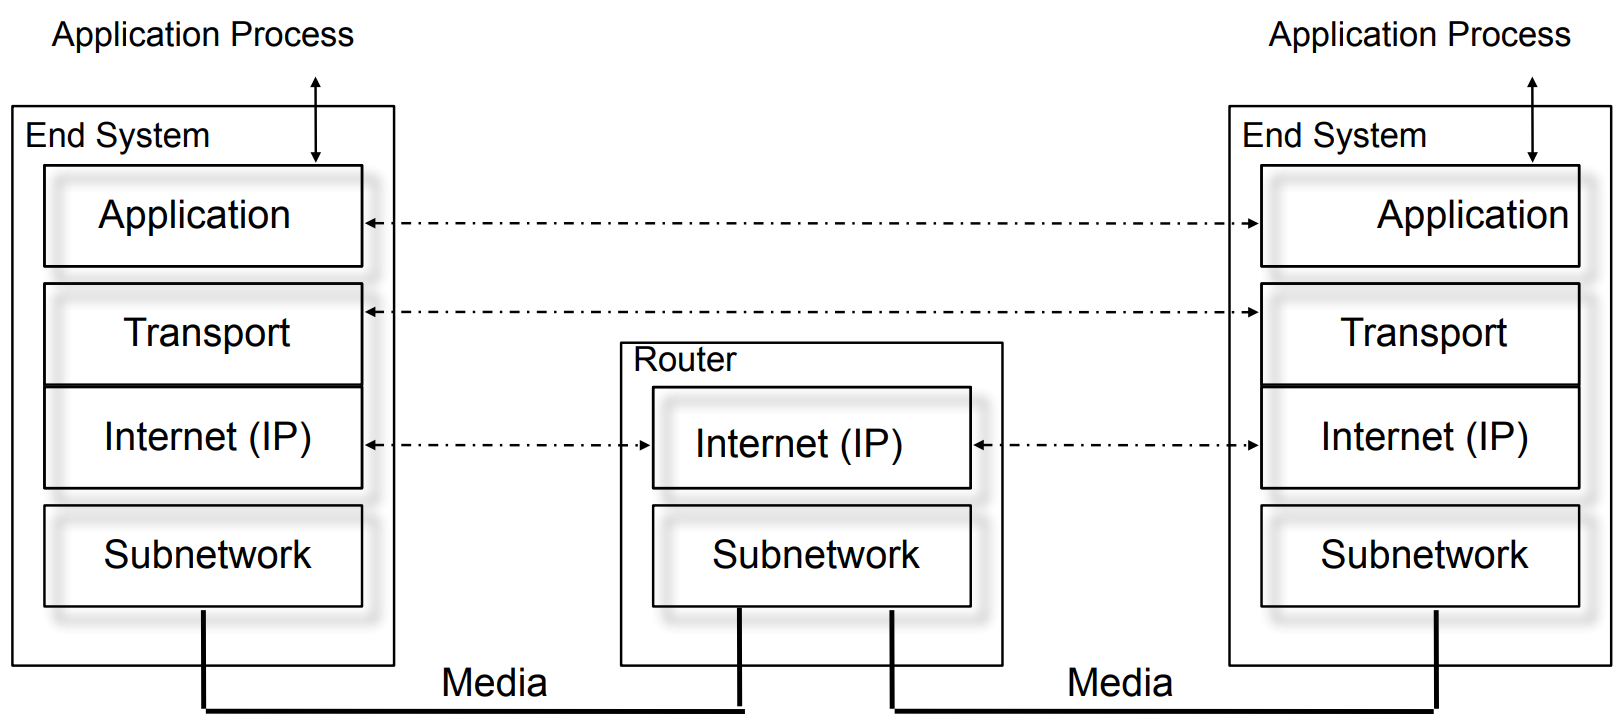
\includegraphics[width=\textwidth]{immagini/Internet_model.png}
\end{figure}

\subsection{Standardization}

\begin{figure}[H]
    \centering
    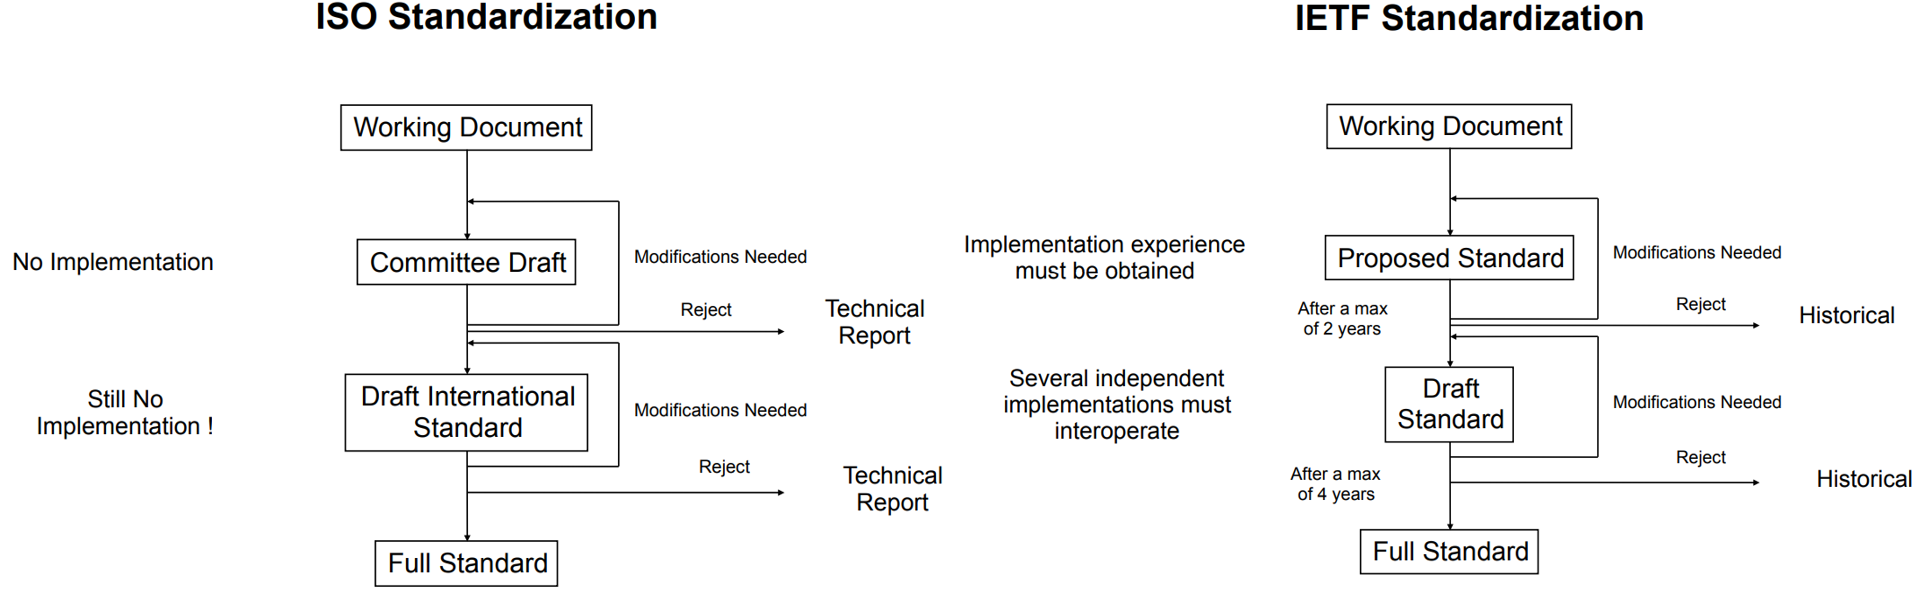
\includegraphics[width=\textwidth]{immagini/Standardization.png}
\end{figure}

\noindent Nella \textbf{ISO standardization} si organizzano un insieme di gruppi di lavoro e si instaura un comitato di persone che discutono del problema da risolvere e dove sporadicamente si eseguono modifiche e si scrivono rapporti.\
Se ciò che si vuole fare non è una buona idea, è possibile eseguire un \textit{technical report}:\ un documento tecnico dove si fa un riassunto delle cose fatte che però sono andate male.\
Quando il comitato si è messo d'accordo, si eseguono i vari draft dello standard all'interno dei quali di passa all'approccio pratico del problema.\
In tutte le fasi della standardizzazione non c'è implementazione ed è quindi possibile che si possano presentare ancora dei problemi una volta arrivati alle fasi finali dello standard.\
Nel corso del tempo verranno poi rilasciate delle patch/fix per andare a risolvere tutti i problemi che ancora non erano stati presi in considerazione.

Nell'\textbf{IETF standardization} l'organizzazione dei processi di standardizzazione è molto diversa:\ innanzitutto si fornisce un timeout (historical) entro il quale l'idea deve essere proseguire, inoltre se il proposed standard va avanti, l'implementazione presentata inizia ad essere testata su più piattaforme (vengono realizzate più implementazioni).\
Nella IETF standardization quindi, quando si arriva a parlare di full standard quest'ultimo è già stato testato più volte (al contrario di come avviene nella standardizzazione OSI).

\section{Overview:\ Abstract Syntax Notation One}

\textbf{Abstract Syntax Notation One} (ASN.1) è una sintassi per la definizione di strutture dati e formati di messaggi.\
Gli obiettivi dell'ASN.1 sono lo scambio di informazioni tra macchine con architetture hardware differenti (8/16/32/64 bit, little/big-endian) e l'indipendenza dai linguaggi di programmazione esistenti (linguaggio neutro).\
Inoltre, la codifica dei dati durante il trasferimento dovrebbe essere selezionabile tra mittenti e destinatari (negoziazione).\
In sostanza, separa la presentazione dei dati dalla rappresentazione della struttura dei dati specifica dell'applicazione:\ la sintassi astratta definisce le strutture dati durante il trasferimento e determina in quale forma queste strutture dati verranno trasferite in serie su una rete.

\begin{figure}[H]
    \centering
    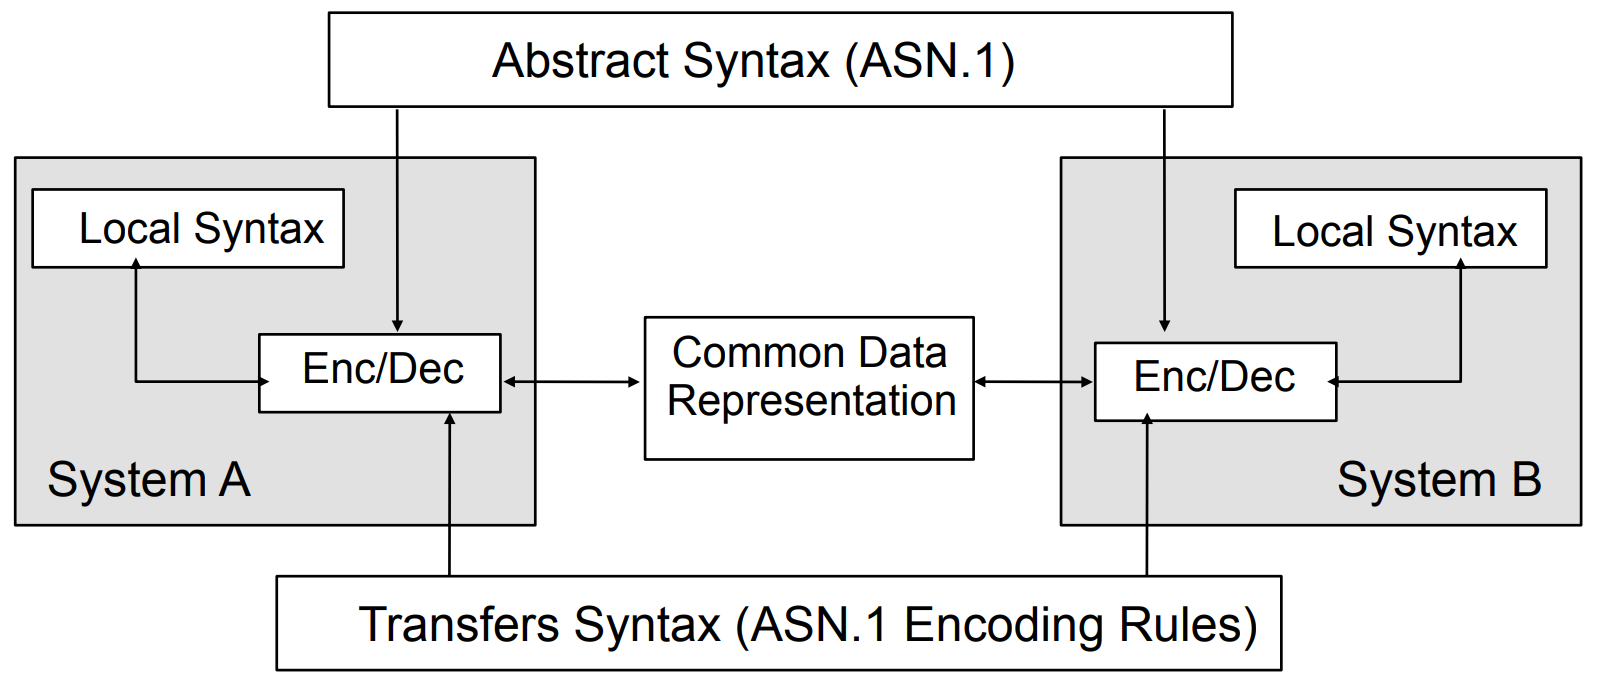
\includegraphics[width=0.8\textwidth]{immagini/ASN.1.png}
\end{figure}

\noindent ASN.1 definisce una sintassi astratta standardizzata; consente diverse regole di codifica che trasformano la sintassi astratta in un flusso di byte adatto al trasferimento.\
\textbf{BER} (\textbf{Basic Encoding Rules}) definisce la mappatura tra sintassi astratta e di trasferimento.\

Le applicazioni normalmente utilizzano una sintassi locale a seconda del linguaggio di programmazione utilizzato.

\subsection{Primitive ASN.1 Datatypes}

I nomi dei tipi di dati ASN.1 iniziano con una lettera maiuscola, mentre i nomi dei valori ASN.1 (costanti) iniziano con una lettera minuscola; le parole chiave ASN.1 e i nomi delle macro sono composti solo da lettere maiuscole.\
I commenti sono racchiusi tra ``-''.

\begin{itemize}
    \item \texttt{BOOLEAN}:\ può assumere solo i valori predefiniti \texttt{TRUE} e \texttt{FALSE}.
    \item \texttt{INTEGER}:\ copre tutti i possibili numeri interi.\ Nessuna delimitazione dell'intervallo di numeri.
    \item \texttt{BIT STRING}:\ una sequenza di bit.\ La lunghezza non deve essere divisibile per 8.
    \item \texttt{OCTET STRING}:\ una sequenza di ottetti (byte).\ È il tipo di base per diversi set di caratteri e altri tipi derivati (\texttt{GeneralizedTime}, \texttt{UTCTime}).
    \item \texttt{ENUMERATED}:\ tipo di enumerazione.\ I valori possibili devono essere determinati dalla definizione dei tipi di dati derivati.
    \item \texttt{OBJECT IDENTIFIER}:\ identificazione univoca di un nodo nell'albero di registrazione ISO.\ Percorso della radice dell'albero al nodo di destinazione.
    \item \texttt{ObjectDescriptor}:\ una stringa di caratteri per l'identificazione di un nodo nell'albero di registrazione.\ Non necessariamente unico.
    \item \texttt{ANY}:\ qualsiasi tipo di dati ASN.1 (unione di tutti i tipi di dati ASN.1, come ``void'' in C).
    \item \texttt{EXTERNAL}:\ dati non descritti utilizzando una definizione ASN.1.
    \item \texttt{NULL}:\ un simbolo sostitutivo, per indicare in un tipo di dati assemblato l'assenza di un valore.
\end{itemize}

\subsubsection{ISO Registration Tree}

Quando si trasferiscono dei dati da un client ad un server, chi fa la richiesta e chi la riceve deve poter comprendere in modo univoco e non ambiguo ciò che gli viene comunicato; ciò è possibile grazie all'ISO Registration Tree:\ viene utilizzato per identificare in modo univoco definizioni, documenti, oggetti, \dots\
Possiede una struttura gerarchica simile ai file system gerarchici, tutti i nodi di un livello identificati da un numero univoco.\
Il percorso dalla radice del Registration Tree a un nodo è una sequenza numerica divisa da punti chiamata \textbf{Object Identifier} (ad esempio 1.3.6.1).

\begin{figure}[H]
    \centering
    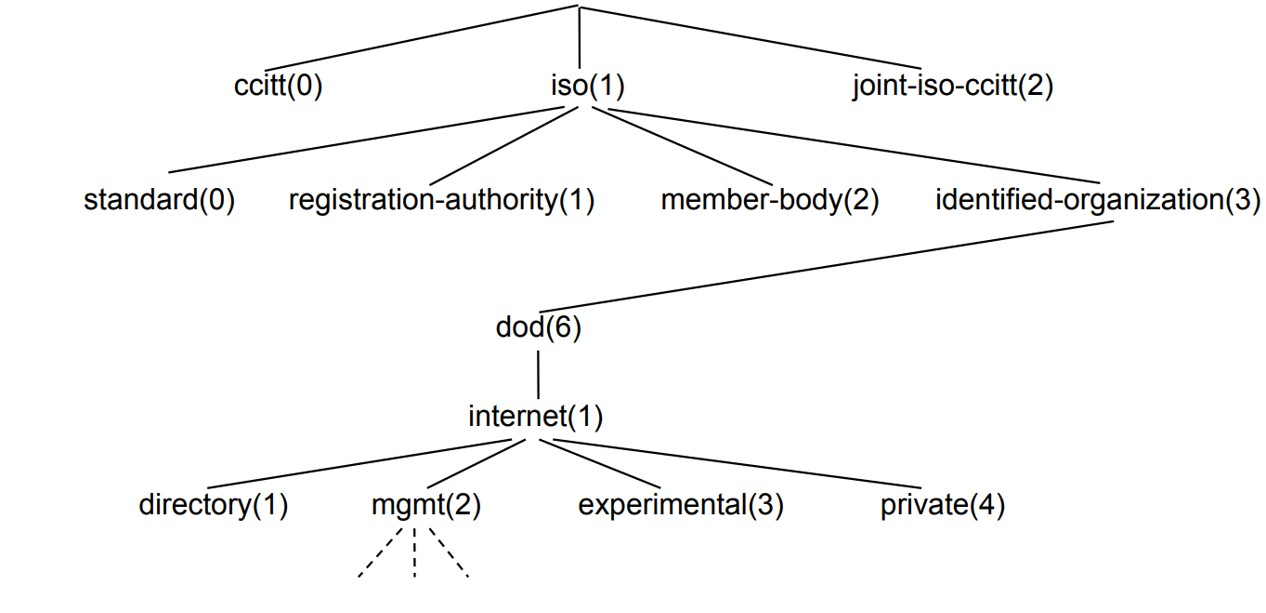
\includegraphics[width=0.8\textwidth]{immagini/ISO_regTree.jpg}
\end{figure}

\subsection{Assembled ASN.1 Datatypes}

A partire dai tipi di base, si possono creare delle composizioni (l'equivalente delle struct in C).\

\begin{itemize}
    \item \texttt{SEQUENCE}:\ corrisponde alle strutture in C o ai record in Pascal.\ La sequenza degli elementi in una \texttt{SEQUENCE} è fissa.
    \item \texttt{SET}:\ simile a \texttt{SEQUENCE}, con la differenza che la sequenza degli elementi non è specificata.
    \item \texttt{SEQUENCE OF}:\ quantità ordinata (elenco) di dati omogenei.
    \item \texttt{SET OF}:\ quantità non ordinata di dati omogenei.
    \item \texttt{CHOICE}:\ tipo di selezione, simile all'union in C.
    \item \texttt{REAL}:\ consiste nel tipo di dati \texttt{INTEGER} esteso con mantissa ed esponente.
\end{itemize}

\subsection{Reduced Datatypes}

Definizione di ulteriori tipi di dati restringendo l'ambito dei tipi di dati esistenti.\
La sintassi esatta dipende dal tipo di dati primitivo sottostante.
\begin{table}[H]
    \centering
    \begin{tabular}{l l l}
        \texttt{LottoNumber} & \texttt{::=} & \texttt{INTEGER (1\dots90)}                   \\
        \texttt{MD5Key}      & \texttt{::=} & \texttt{OCTET STRING (SIZE (16))}             \\
        \texttt{IPAddress}   & \texttt{::=} & \texttt{OCTET STRING (SIZE (4$|$16))}         \\
        \texttt{Counter32}   & \texttt{::=} & \texttt{INTEGER (0\dots4294967295)}           \\
        \texttt{Integer32}   & \texttt{::=} & \texttt{INTEGER (-2147483648\dots2147483647)} \\
        \texttt{Unsigned64}  & \texttt{::=} & \texttt{INTEGER (0\dots18446744073709551615)} \\
    \end{tabular}
\end{table}

\noindent Le limitazioni dell'ambito vengono applicate ai tipi di dati derivati (ad esempio \texttt{SEQUENCE OF MD5Key}).\
La restrizione del tipo di dati \texttt{INTEGER} ha senso in quanto i computer odierni normalmente operano internamente con numeri a 32 o 64 bit.

\subsection{Basic Encoding Rules (BER)}

Le regole di codifica di base determinano come un tipo di dati ASN.1 può essere rappresentato come una stringa di byte e dove ciascuna variabile è identificata da un tag, la lunghezza del valore in byte e il valore di quei byte.\
Tale codifica consente a un destinatario di ricostruire il tipo di un messaggio dal flusso di byte ricevuto.\

La codifica BER è un po' inefficiente poiché spesso ci sono informazioni non necessarie da trasferire; l'uso dei campi \texttt{OPTIONAL} ne ha ulteriormente complicato la definizione.\
Definisce anche la direzione di trasmissione del flusso di bit diversa dalla codifica dei tipi di dati ASN.1:

\begin{figure}[H]
    \centering
    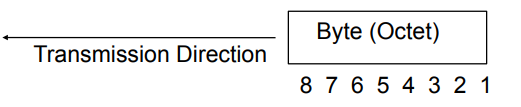
\includegraphics[width=0.5\textwidth]{immagini/BER_direction.png}
\end{figure}

\subsubsection{Coding Tags Classes}

Ogni tag è codificato in un byte:
\begin{figure}[H]
    \centering
    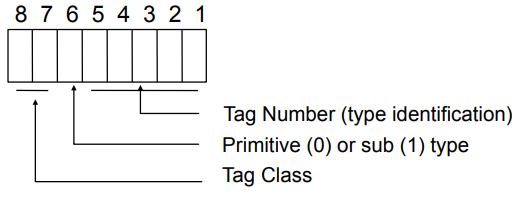
\includegraphics[width=0.5\textwidth]{immagini/BER_tag.png}
\end{figure}

\begin{table}[H]
    \centering
    \begin{tabular}{l c c}
        \multicolumn{3}{c}{\textbf{Tag classes}} \\
                         & Bit 8 & Bit 7         \\
        UNIVERSAL        & 0     & 0             \\
        APPLICATION      & 0     & 1             \\
        CONTEXT-SPECIFIC & 1     & 0             \\
        PRIVATE          & 1     & 1             \\
    \end{tabular}
\end{table}

\subsubsection{Coding Field Length}

Il campo della lunghezza indica la lunghezza del valore immediatamente successivo.\
\begin{itemize}
    \item Lunghezza compresa tra 0\dots127:
          \begin{figure}[H]
              \centering
              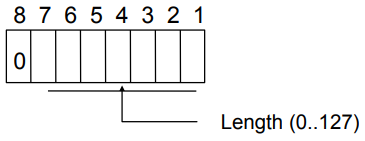
\includegraphics[width=0.4\textwidth]{immagini/BER_lenght1.png}
          \end{figure}
    \item Lunghezza $>$ 127:
          \begin{figure}[H]
              \centering
              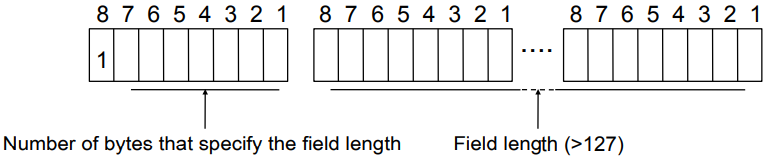
\includegraphics[width=0.7\textwidth]{immagini/BER_lenght2.png}
          \end{figure}
\end{itemize}

\subsubsection{Value Coding}

Per ogni primitivo tipo ASN.1 esiste una regola che consente di tradurre i valori in un flusso di byte e viceversa.\

Le regole per \texttt{INTEGER} e \texttt{OCTET STRING} sono semplici, mentre le regole per \texttt{OBJECT IDENTIFIER} sono relativamente complesse.\
I valori assemblati (\texttt{SEQUENCE}, \texttt{SEQUENCE OF}) sono facilmente rappresentabili codificando ogni singolo elemento.\
Con i costrutti \texttt{CHOICE} viene trasferito solo il valore disponibile, quindi il tag associato deve essere univoco.

La lunghezza della codifica BER deve essere ben nota (nessun valore fittizio) quando viene codificato un valore.\
Con alcune limitazioni è anche possibile specificare la lunghezza dopo il valore.

La decodifica è più difficile quando la lunghezza è specificata dopo il valore.

\begin{verbatim}
30 1B                       SEQUENCE, Length 27
   02 01 00                 INTEGER, Length 1, "0"
   04 06 70 75 62 6C 69 63  OCTET STRING, Length 6, "public"
   A1 0E                    GetNextRequest-PDU, Length 14
      02 04 36 A2 8F 07     INTEGER, Length 4, "916623111"
      02 01 00              INTEGER, Length 1, "0"
      02 01 00              INTEGER, Length 1, "0"
      30 00                 SEQUENCE OF, Length 0
\end{verbatim}

\noindent La codifica dei valori primitivi non è sempre così semplice come nell'esempio (alcuni tipi di dati possono essere codificati sia in forma breve che lunga).
